\documentclass[12pt]{article}
\usepackage{auck2e,multicol,amssymb,amsmath,color}
\usepackage{epsfig}
\usepackage[english]{babel}
\usepackage{blindtext}
\usepackage{microtype}
\usepackage{minted}

%\usepackage{graphicx}
\newcommand{\ds}{\displaystyle}
\newcommand{\mmark}[1]{[{#1 mark(s)}]}
\newcommand{\markk}[1]{[{\bf #1 marks}]}
\newcommand{\dspace}{\renewcommand{\baselinestretch}{2} \small \normalsize}
\newcommand{\sspace}{\renewcommand{\baselinestretch}{1} \small \normalsize}
\newcommand{\btheta}{\mbox{\boldmath $\theta$}}
\newcommand{\blambda}{\mbox{\boldmath $\lambda$}}
\newcommand{\bTheta}{\mbox{\boldmath $\Theta$}}
\newcommand{\bzeta}{\mbox{\boldmath $\zeta$}}
\newcommand{\bpi}{\mbox{\boldmath $\pi$}}
\newcommand{\bphi}{\mbox{\boldmath $\phi$}}
\newcommand{\ba}{\mbox{\boldmath $a$}}
\newcommand{\bb}{\mbox{\boldmath $b$}}
\newcommand{\bd}{\mbox{\boldmath $d$}}
\newcommand{\bm}{\mbox{\boldmath $m$}}
\newcommand{\bx}{\mbox{\boldmath $x$}}
\newcommand{\bh}{\mbox{\boldmath $h$}}
\newcommand{\bu}{\mbox{\boldmath $u$}}
\newcommand{\bP}{\mbox{\boldmath $P$}}
\newcommand{\bQ}{\mbox{\boldmath $Q$}}
\newcommand{\bR}{\mbox{\boldmath $R$}}
\newcommand{\by}{\mbox{\boldmath $y$}}
\newcommand{\bY}{\mbox{\boldmath $Y$}}
\newcommand{\bX}{\mbox{\boldmath $X$}}
\newcommand{\bU}{\mbox{\boldmath $U$}}
\newcommand{\bD}{\mbox{\boldmath $D$}}
\newcommand{\bV}{\mbox{\boldmath $V$}}
\newcommand{\bH}{\mbox{\boldmath $H$}}
\newcommand{\bgamma}{\mbox{\boldmath $\gamma$}}
\newcommand{\bGamma}{\mbox{\boldmath $\Gamma$}}
\newcommand{\balpha}{\mbox{\boldmath $\alpha$}}
\newcommand{\bbeta}{\mbox{\boldmath $\beta$}}
\newcommand{\bdelta}{\mbox{\boldmath $\delta$}}
\newcommand{\bomega}{\mbox{\boldmath $\omega$}}
\newcommand{\bpsi}{\mbox{\boldmath $\psi$}}
\newcommand{\bepsilon}{\mbox{\boldmath $\epsilon$}}
\newcommand{\be}{\begin{eqnarray}}
\newcommand{\ee}{\end{eqnarray}}
\def\BackgroundEPS#1#2#3#4{%
    \special{ps: @beginspecial @setspecial initmatrix
                0.9 setgray #2 #3 translate #4 dup scale}
    \special{ps: plotfile #1}
    \special{ps: @endspecial}
}
\newcommand{\wbugs}{{\sffamily\textbf{WinBUGS }}}
\newcommand{\coda}{{\sffamily\textbf{CODA }}}
\newcommand{\glm}{{\sffamily\textbf{G.L.M }}}
\newcommand{\rwb}{{\sffamily\textbf{R2WinBUGS }}}
\newcommand{\rar}{{\sffamily\textbf{Rock and roll man! }}}
\newcommand{\anova}{{\sffamily\textbf{ANOVA }}}
\newcommand{\mcmc}{{\sffamily\textbf{MCMC }}}
\newcommand{\dic}{{\sffamily\textbf{DIC }}}
\newcommand{\dagr}{{\sffamily\textbf{DAG }}}
\newcommand{\boxeq}[1]{%
\fboxrule=0.5mm%
\fboxsep=5mm%
\begin{center}\fcolorbox{black}{yellow}{\begin{minipage}{0.9\linewidth}
\begin{Beqnarray} #1 \end{Beqnarray}\end{minipage}}\end{center}%
\fboxrule=1pt%
\fboxsep=3pt%
}

\newcommand{\boxst}[1]{%
\fboxrule=0.5mm%
\fboxsep=5mm%
\begin{center}\fcolorbox{black}{yellow}{ \begin{minipage}{0.9\linewidth}#1 \end{minipage} }\end{center}%
\fboxrule=1pt%
\fboxsep=3pt%
}
%%%%%%%%%%%%%%%%%%%%%%%%%%%%%%%%%%%%%%%%%%%%%%%%%%%%%%%%%%%%%%%%%%%%%%%%
% Macro         :   \BackgroundEPS{filename}{tx}{ty}{s}
%-----------------------------------------------------------------------
% Description   :   Display an EPS file in the background of the
%                   current page.
%-----------------------------------------------------------------------
% Author        :   Bernard Desruisseaux (bernard@XYZZYcs.mcgill.ca)
%-----------------------------------------------------------------------
% Usage         :   \BackgroundEPS{pic.eps}{80}{100}{2}
%                   \BackgroundEPS{"`gunzip -c pic.eps.gz"}{80}{100}{2}
%                   \BackgroundEPS{"`zcat pic.eps.Z"}{80}{100}{2}
%%%%%%%%%%%%%%%%%%%%%%%%%%%%%%%%%%%%%%%%%%%%%%%%%%%%%%%%%%%%%%%%%%%%%%%%

\newcommand{\given}{\,|\,}

\paper{Introduction to Bayesian Statistics}
\due{Not for assessment}
\thetitle{\textbf{Tutorial 3}} 
\begin{document}


%\BackgroundEPS{bayes.eps}{0}{0}{1.2}
\makeband


\begin{Questions}

\item The file {\tt shotput.R} contains 
measurements of the weightlifting ability (in kilograms, {\tt data\$x})
and personal best shot put distance (in metres, {\tt data\$y})
for 28 female shot putters. The data, and a model specification
for quadratic regression in JAGS, are given below.

\begin{figure}[!ht]
\centering
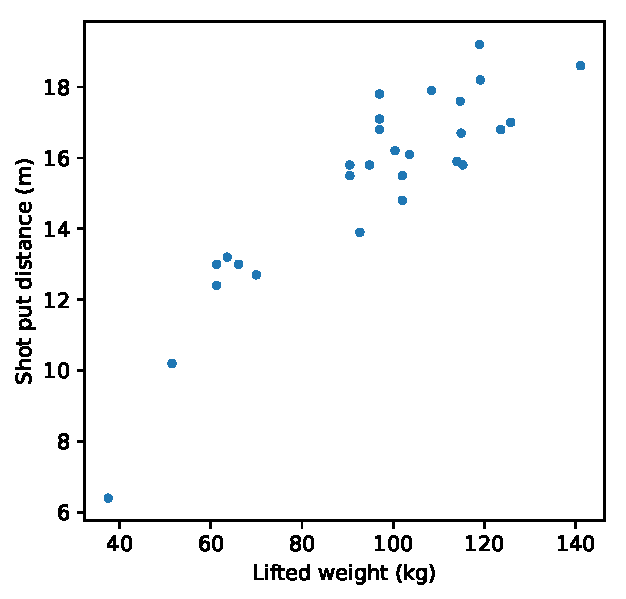
\includegraphics[width=0.5\textwidth]{shotput.pdf}
\end{figure}

% http://www.stat.ufl.edu/~winner/

\begin{minted}{r}
model
{
    beta0 ~ dunif(-1000, 1000)
    beta1 ~ dunif(-1000, 1000)
    beta2 ~ dunif(-1000, 1000)
    log_sigma ~ dunif(-10, 10)
    sigma <- exp(log_sigma)

    for(i in 1:N)
    {
        mu[i] <- beta0 + beta1*(x[i] - mean(x)) + beta2*(x[i] - mean(x))^2
        y[i] ~ dnorm(mu[i], 1/sigma^2)
    }
}
\end{minted}
Note that the $x$-values in the regression model are `centered',
i.e., the average is subtracted. The main advantage of this is the
interpretation of $\beta_0$ improves. It is now the typical shot put distance
that would occur for an average weightlifter. Without subtracting the mean,
$\beta_0$ would have meant the typical shot distance for a weightlifting
result of zero, which is much harder to understand and assign a prior to.

\begin{enumerate}
\item [(a)] The priors in the model are standard and convenient, but actually
represent fairly ridiculous prior beliefs about shotput and weightlifting.
Consider $\beta_0$ in particular, which is in units of metres.
State one way in which the Uniform$(-1000, 1000)$ prior is not realistic.
Then suggest an alternative prior for $\beta_0$ which is based on reasonable judgments
about shotput distance.
However, do not change the JAGS code to implement your alternative prior.

\item [(b)] Run JAGS for a standard number of iterations.
                Plot trace plots and make sure they look healthy.
\item [(c)] Look at the marginal posterior distributions for
$\beta_0$, $\beta_1$, and $\sigma$, and calculate a credible interval for
each of these.
\item [(d)] Looking at the data,
                it looks like the degree
                of scatter also increases as $x$ increases. Suppose that
                the standard deviation of the sampling distribution
                is $\sigma \exp(kx)$, instead of
                just $\sigma$, where $k$ is some constant. Modify the model
                accordingly
                by adding a line
    \mintinline{r}{sigma_obs[i] <- sigma*exp(k*x[i])}
    and using \mintinline{r}{sigma_obs[i]} in the likelihood instead of
        \mintinline{r}{sigma}.
     Give $k$ a Uniform$(-1, 1)$ prior.

\item [(e)] Run JAGS with the change from part (d).
Calculate the posterior
probability that $k$ is positive, i.e., that the noise is really increasing
with $x$.
\end{enumerate}

\item
The British fire brigade keeps track of the number of
calls each year from people stuck in household items. The Poisson distribution
is an appropriate model for counts of rare events. The data are:
\begin{verbatim}
data = list(t=c(0, 1, 2), y=c(416, 441, 453), N=3)
\end{verbatim}
and we will use the following JAGS model, which is a traditional `GLM'
`Poisson regression' model, with naive priors.

\begin{minted}{r}
model
{
    beta0 ~ dunif(-1000, 1000)
    beta1 ~ dunif(-1000, 1000)

    for(i in 1:N)
    {
        mu[i] <- exp(beta0 + beta1*(t[i] - mean(t)))
        y[i] ~ dpois(mu[i])
    }
}
\end{minted}

The fire brigade wants to know whether there is evidence of a real increase
over time, or whether the apparent trend is just due to fluctuations and will
not continue into the future. See
\url{http://www.statschat.org.nz/2013/07/30/always-ask-for-the-margin-of-error/}
for the context behind this question\footnote{Professor Thomas Lumley called the evidence
for a real increasing trend ``very unimpressive''. In my opinion the evidence for
a real increase is weak but not negligible.}.

\begin{enumerate}
\item [(a)] Run the model for enough steps that the trace plots look good and
exclude any burn-in if necessary.
Find the posterior probability that $\beta_1 > 0$, i.e. that the ``real'' trend
is upwards.
\item [(b)] Calculate the posterior mean of $\beta_1$ and a 95\% credible interval.
\item [(c)] Change the prior on $\beta_1$ to a {\tt dt(0, 1/0.01\^{ }2, 1)} distribution (meaning
we expect the rate of change to be small, probably less than a few \% per year, but with
heavy tailed prior uncertainty).
\item [(d)] With the new prior, find the posterior probability that $\beta_1 > 0$.
\item [(e)] Add a JAGS node and find the posterior predictive probability
that in the next year ($t=3$), the count of these incidents will be higher than
the average of the data so far (436.67).
\end{enumerate}

\item
{\bf Note}: This question is harder, because I'm getting you to write the
whole model from scratch, based on the story being told. This is common
in applied Bayesian work --- it is rare that a scientific situation exactly
matches a standard model.
I am happy to help out as much as necessary.

The file {\tt solar\_simplified.csv}
contains information about the amount
of solar energy generated (in kilowatt-hours) each day at my house,
since we had the panels installed in March 2026. The beginning of the data
looks like this:
\begin{minted}{r}
> data = read.csv("solar_simplified.csv")
> head(data)
  t     y
1 1 30.00
2 2 26.38
3 3 34.27
4 4 33.16
5 5 25.05
6 6  7.15
\end{minted}
The first column (\mintinline{r}{t}) is the day, and the second 
column (\mintinline{r}{y}) is the electricity production that day
in kilowatt-hours. The data is plotted below.

\begin{center}
\includegraphics[width=0.7\textwidth]{solar.pdf}
\end{center}

Consider a model where the maximum possible production
(if clouds did not exist) varies over the year
according to a sine wave:
\begin{align}
y_{\rm max}(t)
    &= C + A\sin\left(\frac{2\pi t}{365.25} + \phi\right).
\end{align}
The constant $C$ scales the typical production over the whole year
(if clouds did not exist).
The amplitude parameter $A$ describes how strongly production
varies over the year (i.e., if $A$ is large, summer and winter are
more different). The period of the sine wave is already known to
be 365.25 days, and the phase parameter $\phi$ determines when the
minimum and maximum will occur in terms of the time variable \mintinline{r}{t}.

Due to clouds, the actual production \mintinline{r}{y} on day
$t$ will be less than $y_{\rm max}(t)$. Assume that the actual
production is given by a truncated normal distribution peaking at
$ky_{\rm max}(t)$, where $k$ is some parameter between 0 and 1.
The parameter $k$ describes the effect of clouds. If $k$ were close to
1 then production would always be near the maximum and clouds aren't
doing much. If $k$ is closer to zero then clouds are blocking most of
the production.

Let the width of the normal distribution be
$\sigma k y_{\rm max}(t)$, where $\sigma$ is an unknown parameter,
also between 0 and 1. This makes the day to day variation in production
proportional to the typical production $k y_{\rm max}$, with $\sigma$
as the proportionality constant.

The normal distribution will also be truncated to be between
$0$ and $y_{\rm max}$. Overall, the sampling distribution is
\begin{align}
y_t &\sim \textnormal{Normal}
            \left(ky_{\rm max}(t), \left(\sigma k y_{\rm max}(t)\right)^2\right)
            T(0, y_{\rm max}(t)).\label{eqn:likelihood}
\end{align}
where $T()$ at the end represents truncation (cutting off the edges of the
distribution).

\begin{enumerate}
\item [(a)] Write down the JAGS code to implement the likelihood part of
the model. {\bf Hint}: JAGS accepts truncation notation using \mintinline{r}{T()}
written just after the distribution, just like in Equation~\ref{eqn:likelihood}.
\item [(b)] Assume the following priors for $k$, $\sigma$, $\phi$, and $C$:
\begin{align}
k &\sim \textnormal{Uniform}(0, 1) \\
\sigma &\sim \textnormal{Uniform}(0, 1) \\
\phi &\sim \textnormal{Uniform}(0, 2\pi) \\
C &\sim \textnormal{Uniform}(0, 100).
\end{align}
For the amplitude parameter $A$, we need to ensure that $y_{\rm max}(t)$
can never be negative. If $A$ is less than $C$, this will be guaranteed,
because the sine function cannot be less than $-1$, and the minimum
of $y_{\rm max}$, which is $A - C$, will never
be negative.
Thus, let the prior for $A$ be dependent on $C$:
\begin{align}
A &\sim \textnormal{Uniform}(0, C).
\end{align}
Write down the JAGS code for the priors.
\item [(c)] Run JAGS for 100,000 iterations with \mintinline{r}{thin = 10}.
This might take a few minutes. Check the trace plots to make sure everything
worked sufficiently well. If there is any significant burn-in period, remove it
from the results.
{\bf Note}: In this model it is possible for some parameter values to be
completely ruled out by the data, because the sine curve has to be above all
the data points. JAGS complains if its starting values for the parameters
are completely impossible given the data. Sometimes you need to pass
different \mintinline{r}{inits} to JAGS to specify the starting values of
the parameters. If it seems like you need to do this, here is the line to
modify:
\begin{minted}{r}
jm = jags.model(textConnection(model), data,
                        inits=list(list(k=0.5, phi=1, C=99, A=1)))
\end{minted}
\item[(d)] Plot the posterior for \mintinline{r}{k} and comment on the
effect of clouds on solar production in Kumeū.

\item [(e)] Plot the data using
\mintinline{r}{plot(data$t, data$y, type="l", xlim=c(0, 365), ylim=c(0, 80))}.
The xlim and ylim are to enlarge the range of the plot so you can do the
next step.
Overplot ten curves $y_{\rm max}(t)$ using parameter values from the
posterior samples, to show what the maximum production could look like over
the year (including summer which hasn't happened yet).
Note: All of the ten curves should be just
above the data, not going through it.

\item [(f)] The theoretical maximum production at the height of summer
with zero clouds is $C + A$. Plot the posterior distribution for $C + A$.
You can either use your existing posterior samples or add a deterministic
node to JAGS to represent this and run JAGS again.

\end{enumerate}



\end{Questions}

\end{document}




